\documentclass{article}
\usepackage{tikz}
\usepackage{amsmath}
\usepackage{ctex}
\usepackage{xcolor}
\usetikzlibrary {positioning}
\title{一种基于口胡的KMP算法介绍(雾)}
\author{周致远}
\begin{document}
	\maketitle
	
	众所周知,字符串模式匹配是计算机科学最为古老的问题之一。朴素的字符串匹配算法可以描述为:对于待匹配字符串(下称之为文本)的每一个位置,逐个字符比较从该位置开始是否与模式串(下称之为子串)完全匹配。时间复杂度为$O(n*m)$,十分低效。于是,我接下来要介绍一种更快、更优雅,而且基本是线性复杂度的字符串匹配算法——KMP算法(The Knuth-Morris-Pratt Algorithm)。

	KMP的思想是充分利用朴素算法忽略的信息来加快匹配。假设有如下文本:

	$$goodgoogle$$

	和以下子串:

	$$google$$


	则朴素的方法可表示为:\\

	\begin{centering}
	\usetikzlibrary {arrows.meta, positioning}
	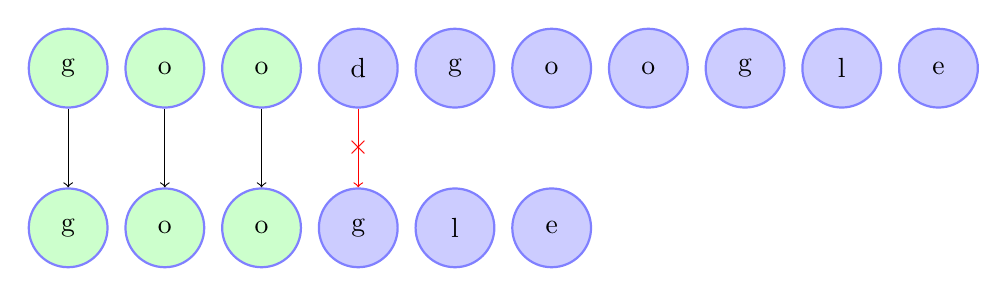
\begin{tikzpicture}
		[place/.style={circle,draw=blue!50,fill=blue!20,thick,inner sep=0pt, minimum size=10mm},
		correct/.style={circle,draw=blue!50,fill=green!20,thick,inner sep=0pt, minimum size=10mm},
		transition/.style={rectangle,draw=black!50,fill=black!20,thick, inner sep=0pt, minimum size=6mm}]
		\node [correct] (b1) {g};
		\node [correct] (b2) [right=2mm of b1]{o};
		\node [correct] (b3) [right=2mm of b2]{o};
		\node [place] (b4) [right=2mm of b3]{d};
		\node [place] (b5) [right=2mm of b4]{g};
		\node [place] (b6) [right=2mm of b5]{o};
		\node [place] (b7) [right=2mm of b6]{o};
		\node [place] (b8) [right=2mm of b7]{g};
		\node [place] (b9) [right=2mm of b8]{l};
		\node [place] (b10) [right=2mm of b9]{e};

		\node [correct] (a1) [below =of b1]{g};
		\node [correct] (a2) [right=2mm of a1]{o};
		\node [correct] (a3) [right=2mm of a2]{o};
		\node [place] (a4) [right=2mm of a3]{g};
		\node [place] (a5) [right=2mm of a4]{l};
		\node [place] (a6) [right=2mm of a5]{e};

		\draw [->] (b1) to (a1);
		\draw [->] (b2) to (a2);
		\draw [->] (b3) to (a3);
		\draw [red, ->] (b4) -- (a4) node [midway] {$\times$};

	\end{tikzpicture}
	\end{centering}

	\vspace{1cm}

	\begin{centering}
	\usetikzlibrary {arrows.meta, positioning}
	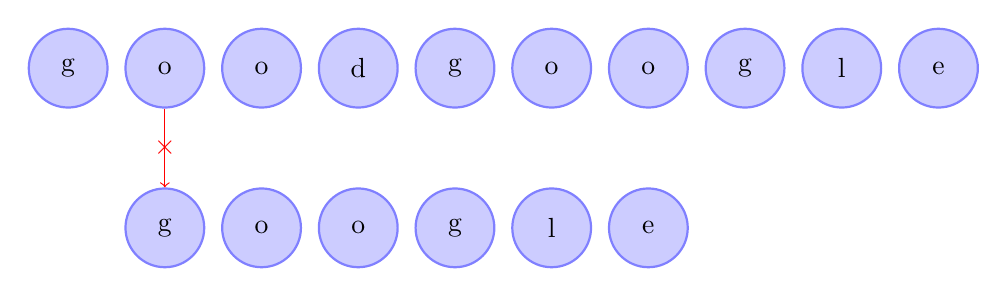
\begin{tikzpicture}
		[place/.style={circle,draw=blue!50,fill=blue!20,thick,inner sep=0pt, minimum size=10mm},
		correct/.style={circle,draw=blue!50,fill=green!20,thick,inner sep=0pt, minimum size=10mm},
		transition/.style={rectangle,draw=black!50,fill=black!20,thick, inner sep=0pt, minimum size=6mm}]
		\node [place] (b1) {g};
		\node [place] (b2) [right=2mm of b1]{o};
		\node [place] (b3) [right=2mm of b2]{o};
		\node [place] (b4) [right=2mm of b3]{d};
		\node [place] (b5) [right=2mm of b4]{g};
		\node [place] (b6) [right=2mm of b5]{o};
		\node [place] (b7) [right=2mm of b6]{o};
		\node [place] (b8) [right=2mm of b7]{g};
		\node [place] (b9) [right=2mm of b8]{l};
		\node [place] (b10) [right=2mm of b9]{e};

		\node [place] (a1) [below =of b2]{g};
		\node [place] (a2) [right=2mm of a1]{o};
		\node [place] (a3) [right=2mm of a2]{o};
		\node [place] (a4) [right=2mm of a3]{g};
		\node [place] (a5) [right=2mm of a4]{l};
		\node [place] (a6) [right=2mm of a5]{e};

		\draw [red, ->] (b2) -- (a1) node [midway] {$\times$};

	\end{tikzpicture}
	\end{centering}

	\vspace{1cm}

	\begin{centering}
	\usetikzlibrary {arrows.meta, positioning}
	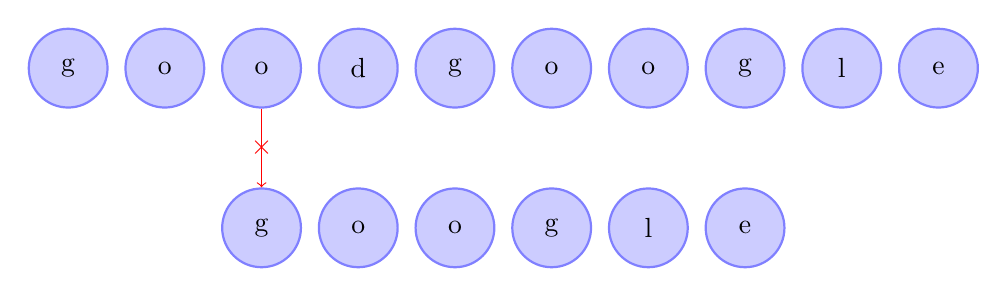
\begin{tikzpicture}
		[place/.style={circle,draw=blue!50,fill=blue!20,thick,inner sep=0pt, minimum size=10mm},
		correct/.style={circle,draw=blue!50,fill=green!20,thick,inner sep=0pt, minimum size=10mm},
		transition/.style={rectangle,draw=black!50,fill=black!20,thick, inner sep=0pt, minimum size=6mm}]
		\node [place] (b1) {g};
		\node [place] (b2) [right=2mm of b1]{o};
		\node [place] (b3) [right=2mm of b2]{o};
		\node [place] (b4) [right=2mm of b3]{d};
		\node [place] (b5) [right=2mm of b4]{g};
		\node [place] (b6) [right=2mm of b5]{o};
		\node [place] (b7) [right=2mm of b6]{o};
		\node [place] (b8) [right=2mm of b7]{g};
		\node [place] (b9) [right=2mm of b8]{l};
		\node [place] (b10) [right=2mm of b9]{e};

		\node [place] (a1) [below =of b3]{g};
		\node [place] (a2) [right=2mm of a1]{o};
		\node [place] (a3) [right=2mm of a2]{o};
		\node [place] (a4) [right=2mm of a3]{g};
		\node [place] (a5) [right=2mm of a4]{l};
		\node [place] (a6) [right=2mm of a5]{e};

		\draw [red, ->] (b3) -- (a1) node [midway] {$\times$};

	\end{tikzpicture}
	\end{centering}

	$$ 2\  steps\  later ... $$

	\vspace{0.7cm}

	\begin{centering}
	\usetikzlibrary {arrows.meta, positioning}
	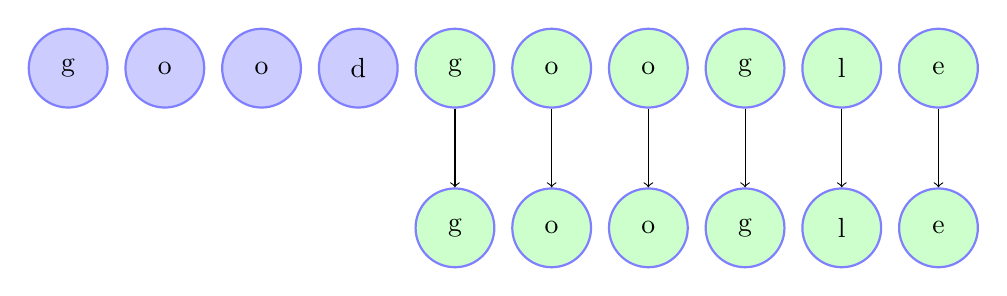
\begin{tikzpicture}
		[place/.style={circle,draw=blue!50,fill=blue!20,thick,inner sep=0pt, minimum size=10mm},
		correct/.style={circle,draw=blue!50,fill=green!20,thick,inner sep=0pt, minimum size=10mm},
		transition/.style={rectangle,draw=black!50,fill=black!20,thick, inner sep=0pt, minimum size=6mm}]
		\node [place] (b1) {g};
		\node [place] (b2) [right=2mm of b1]{o};
		\node [place] (b3) [right=2mm of b2]{o};
		\node [place] (b4) [right=2mm of b3]{d};
		\node [correct] (b5) [right=2mm of b4]{g};
		\node [correct] (b6) [right=2mm of b5]{o};
		\node [correct] (b7) [right=2mm of b6]{o};
		\node [correct] (b8) [right=2mm of b7]{g};
		\node [correct] (b9) [right=2mm of b8]{l};
		\node [correct] (b10) [right=2mm of b9]{e};

		\node [correct] (a1) [below =of b5]{g};
		\node [correct] (a2) [right=2mm of a1]{o};
		\node [correct] (a3) [right=2mm of a2]{o};
		\node [correct] (a4) [right=2mm of a3]{g};
		\node [correct] (a5) [right=2mm of a4]{l};
		\node [correct] (a6) [right=2mm of a5]{e};

		\draw [->] (b5) -- (a1);
		\draw [->] (b6) -- (a2);
		\draw [->] (b7) -- (a3);
		\draw [->] (b8) -- (a4);
		\draw [->] (b9) -- (a5);
		\draw [->] (b10) -- (a6);

	\end{tikzpicture}
	\end{centering}

	设文本表示为 $\{s_1, s_2 , ... , s_10\}$;子串表示为 $\{t_1, t_2, ... , t_6\}$(下同),
	我们发现,即便出现三个字符"goo"="goo"匹配的特殊情况,朴素算法也会无视这一点,直接跳到文本下一位和子串初始位。实际上,其中仍有可挖掘的信息:部分匹配给予了算法关于文本的一部分知识。基于朴素匹配算法,设子串长度为n,文本长度为$n_t$,如果把子串看成一个n维向量:

	$$ T = 
	\left[\begin{array}{c} 
			\color{green!50!black}\mathbf{g} \\ 
			\color{green!50!black}\mathbf{o} \\
			\color{green!50!black}\mathbf{o} \\
			g \\ 
			l \\
			e
	\end{array}\right]
	$$

	把朴素算法匹配文本的过程看成n维空间:

	$$
	S = 
	\left[\begin{array}{cccccc}
			\color{green!50!black}\mathbf{g} & \color{green!50!black}\mathbf{o} & \color{green!50!black}\mathbf{o} & d & g & o \\
			o&o&d&g&o&o \\ 
			o&d&g&o&o&g \\
			d&g&o&o&g&l \\
			g&o&o&g&l&e 
	\end{array}\right]
	$$
	
	字符串模式匹配$S \times T$过程中观察矩阵$S$,第一行已经匹配出"goo",接下来要匹配的几行的前三个字符与"goo"都不完全相同:

	$$
	\left[\begin{array}{cccccc}
			\color{green!50!black}\mathbf{g} & \color{green!50!black}\mathbf{o} & \color{green!50!black}\mathbf{o} & d & g & o \\
			\color{red}\mathbf{o}&\color{red}\mathbf{o}&\color{blue}\mathbf{d}&g&o&o \\ 
			\color{red}\mathbf{o}&\color{blue}\mathbf{d}&\color{blue}\mathbf{g}&o&o&g \\
			\color{blue}\mathbf{d}&\color{blue}\mathbf{g}&\color{blue}\mathbf{o}&o&g&l \\
			g&o&o&g&l&e 
	\end{array}\right]
	$$

	标为红色的元素是在部分匹配时就已经确定了的,这意味着算法如果能根据已知的红色信息跳过部分匹配长度的匹配次数,就可以将复杂度降到线性!并且部分匹配的字符串还有一个更加优良的特性:它是子串的一部分,也就是说可以根据部分匹配的长度+子串信息就可以判断跳过哪些匹配。根据红色部分已知信息,下一次跳过取决于:

	\vspace{0.7cm}

	%此时我们已知在当前位置,文本和子串的前三位相等且为"goo";而下一次匹配时的前两位为"oo",再下一次匹配的前一位为"o",这就是我们根据相等获得的额外信息。所以,只要"go"!="oo"则可以跳过下一条、"g"!="o"则可以跳过再下一条,可惜再下次匹配的前三位已经不包含任何第一次的字符了,根据已知信息已经无法跳过更多匹配,于是在这停顿。

	\begin{centering}
	\usetikzlibrary {arrows.meta, positioning}
	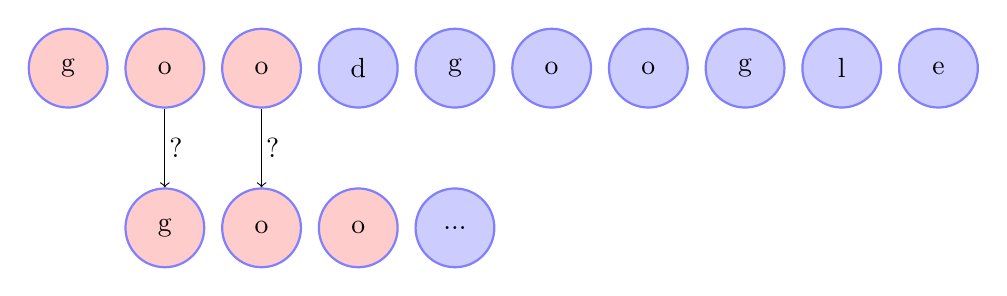
\begin{tikzpicture}
		[place/.style={circle,draw=blue!50,fill=blue!20,thick,inner sep=0pt, minimum size=10mm},
		correct/.style={circle,draw=blue!50,fill=red!20,thick,inner sep=0pt, minimum size=10mm},
		transition/.style={rectangle,draw=black!50,fill=black!20,thick, inner sep=0pt, minimum size=6mm}]
		\node [correct] (b1) {g};
		\node [correct] (b2) [right=2mm of b1]{o};
		\node [correct] (b3) [right=2mm of b2]{o};
		\node [place] (b4) [right=2mm of b3]{d};
		\node [place] (b5) [right=2mm of b4]{g};
		\node [place] (b6) [right=2mm of b5]{o};
		\node [place] (b7) [right=2mm of b6]{o};
		\node [place] (b8) [right=2mm of b7]{g};
		\node [place] (b9) [right=2mm of b8]{l};
		\node [place] (b10) [right=2mm of b9]{e};

		\node [correct] (a1) [below =of b2]{g};
		\node [correct] (a2) [right=2mm of a1]{o};
		\node [correct] (a3) [right=2mm of a2]{o};
		\node [place] (a4) [right=2mm of a3]{...};

		\draw [->] (b2) -- (a1) node [midway, xshift = 4]{?};
		\draw [->] (b3) -- (a2) node [midway, xshift = 4] {?};

	\end{tikzpicture}
	\end{centering}
	
	此处仅涉及已知量(红色);那么再下一次匹配是否跳过取决于:

	\vspace{0.5cm}

	\begin{centering}
	\usetikzlibrary {arrows.meta, positioning}
	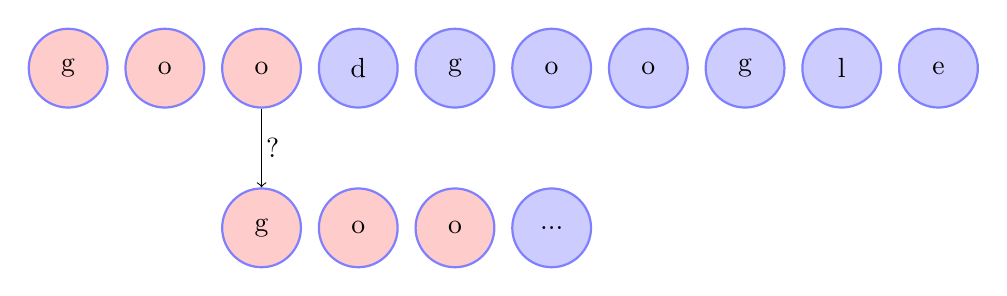
\begin{tikzpicture}
		[place/.style={circle,draw=blue!50,fill=blue!20,thick,inner sep=0pt, minimum size=10mm},
		correct/.style={circle,draw=blue!50,fill=red!20,thick,inner sep=0pt, minimum size=10mm},
		transition/.style={rectangle,draw=black!50,fill=black!20,thick, inner sep=0pt, minimum size=6mm}]
		\node [correct] (b1) {g};
		\node [correct] (b2) [right=2mm of b1]{o};
		\node [correct] (b3) [right=2mm of b2]{o};
		\node [place] (b4) [right=2mm of b3]{d};
		\node [place] (b5) [right=2mm of b4]{g};
		\node [place] (b6) [right=2mm of b5]{o};
		\node [place] (b7) [right=2mm of b6]{o};
		\node [place] (b8) [right=2mm of b7]{g};
		\node [place] (b9) [right=2mm of b8]{l};
		\node [place] (b10) [right=2mm of b9]{e};

		\node [correct] (a1) [below =of b3]{g};
		\node [correct] (a2) [right=2mm of a1]{o};
		\node [correct] (a3) [right=2mm of a2]{o};
		\node [place] (a4) [right=2mm of a3]{...};

		\draw [->] (b3) -- (a1) node [midway, xshift = 4]{?};

	\end{tikzpicture}
	\end{centering}

	在子串滑动的过程中,我们惊讶的发现每次判断是否跳过时,其实是在判断已知部分的前后缀是否相等!(找回了前世记忆)而这就是KMP算法的主要思想所在。让我们再看一组例子:

	\vspace{0.5cm}

	\begin{centering}
	\usetikzlibrary {arrows.meta, positioning}
	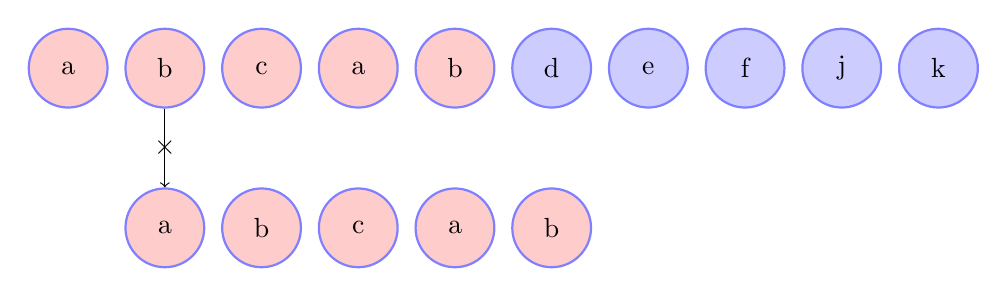
\begin{tikzpicture}
		[place/.style={circle,draw=blue!50,fill=blue!20,thick,inner sep=0pt, minimum size=10mm},
		correct/.style={circle,draw=blue!50,fill=red!20,thick,inner sep=0pt, minimum size=10mm},
		transition/.style={rectangle,draw=black!50,fill=black!20,thick, inner sep=0pt, minimum size=6mm}]
		\node [correct] (b1) {a};
		\node [correct] (b2) [right=2mm of b1]{b};
		\node [correct] (b3) [right=2mm of b2]{c};
		\node [correct] (b4) [right=2mm of b3]{a};
		\node [correct] (b5) [right=2mm of b4]{b};
		\node [place] (b6) [right=2mm of b5]{d};
		\node [place] (b7) [right=2mm of b6]{e};
		\node [place] (b8) [right=2mm of b7]{f};
		\node [place] (b9) [right=2mm of b8]{j};
		\node [place] (b10) [right=2mm of b9]{k};

		\node [correct] (a1) [below =of b2]{a};
		\node [correct] (a2) [right=2mm of a1]{b};
		\node [correct] (a3) [right=2mm of a2]{c};
		\node [correct] (a4) [right=2mm of a3]{a};
		\node [correct] (a5) [right=2mm of a4]{b};

		\draw [->] (b2) -- (a1) node [midway]{$\times$};

	\end{tikzpicture}
	\end{centering}

	
	\vspace{0.5cm}

	\begin{centering}
	\usetikzlibrary {arrows.meta, positioning}
	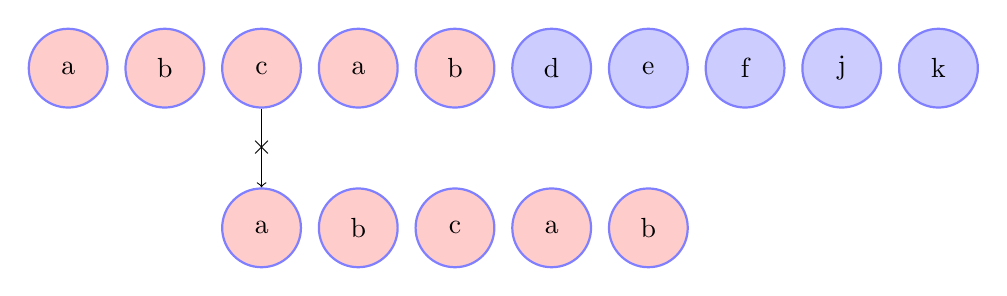
\begin{tikzpicture}
		[place/.style={circle,draw=blue!50,fill=blue!20,thick,inner sep=0pt, minimum size=10mm},
		correct/.style={circle,draw=blue!50,fill=red!20,thick,inner sep=0pt, minimum size=10mm},
		transition/.style={rectangle,draw=black!50,fill=black!20,thick, inner sep=0pt, minimum size=6mm}]
		\node [correct] (b1) {a};
		\node [correct] (b2) [right=2mm of b1]{b};
		\node [correct] (b3) [right=2mm of b2]{c};
		\node [correct] (b4) [right=2mm of b3]{a};
		\node [correct] (b5) [right=2mm of b4]{b};
		\node [place] (b6) [right=2mm of b5]{d};
		\node [place] (b7) [right=2mm of b6]{e};
		\node [place] (b8) [right=2mm of b7]{f};
		\node [place] (b9) [right=2mm of b8]{j};
		\node [place] (b10) [right=2mm of b9]{k};

		\node [correct] (a1) [below =of b3]{a};
		\node [correct] (a2) [right=2mm of a1]{b};
		\node [correct] (a3) [right=2mm of a2]{c};
		\node [correct] (a4) [right=2mm of a3]{a};
		\node [correct] (a5) [right=2mm of a4]{b};

		\draw [->] (b3) -- (a1) node [midway]{$\times$};

	\end{tikzpicture}
	\end{centering}

	
	\vspace{0.5cm}

	\begin{centering}
	\usetikzlibrary {arrows.meta, positioning}
	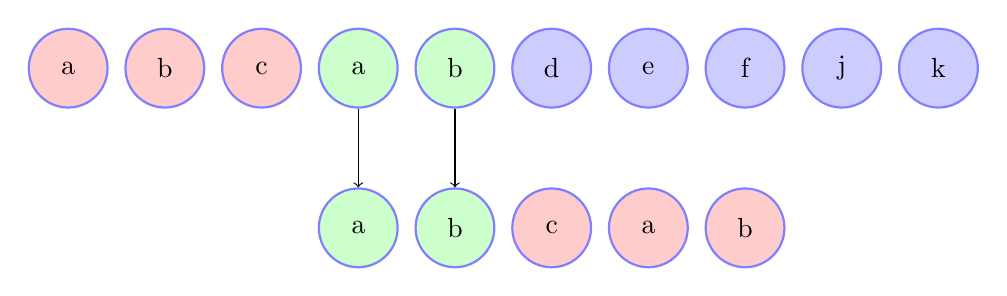
\begin{tikzpicture}
		[place/.style={circle,draw=blue!50,fill=blue!20,thick,inner sep=0pt, minimum size=10mm},
		correct/.style={circle,draw=blue!50,fill=red!20,thick,inner sep=0pt, minimum size=10mm},
		correct2/.style={circle,draw=blue!50,fill=green!20,thick,inner sep=0pt, minimum size=10mm},
		transition/.style={rectangle,draw=black!50,fill=black!20,thick, inner sep=0pt, minimum size=6mm}]
		\node [correct] (b1) {a};
		\node [correct] (b2) [right=2mm of b1]{b};
		\node [correct] (b3) [right=2mm of b2]{c};
		\node [correct2] (b4) [right=2mm of b3]{a};
		\node [correct2] (b5) [right=2mm of b4]{b};
		\node [place] (b6) [right=2mm of b5]{d};
		\node [place] (b7) [right=2mm of b6]{e};
		\node [place] (b8) [right=2mm of b7]{f};
		\node [place] (b9) [right=2mm of b8]{j};
		\node [place] (b10) [right=2mm of b9]{k};

		\node [correct2] (a1) [below =of b4]{a};
		\node [correct2] (a2) [right=2mm of a1]{b};
		\node [correct] (a3) [right=2mm of a2]{c};
		\node [correct] (a4) [right=2mm of a3]{a};
		\node [correct] (a5) [right=2mm of a4]{b};

		\draw [->] (b4) -- (a1) node [midway, xshift = 4]{};
		\draw [->] (b5) -- (a2) node [midway, xshift = 4]{};

	\end{tikzpicture}
	\end{centering}

	也即,此时满足:

	\begin{centering}
	\usetikzlibrary {arrows.meta, positioning}
	\begin{tikzpicture}[bend angle=45,
		place/.style={circle,draw=blue!50,fill=blue!20,thick,inner sep=0pt, minimum size=10mm},
		correct/.style={circle,draw=blue!50,fill=red!20,thick,inner sep=0pt, minimum size=10mm},
		correct2/.style={circle,draw=blue!50,fill=green!20,thick,inner sep=0pt, minimum size=10mm},
		transition/.style={rectangle,draw=black!50,fill=black!20,thick, inner sep=0pt, minimum size=6mm}]

		\node [correct] (a3) {c};
		\node [correct2] (a4) [right=2mm of a3]{a};
		\node [correct2] (a5) [right=2mm of a4]{b};

		\node [correct2] (a2) [left=2mm of a3]{b}
			edge [pre, bend left] (a5);
		\node [correct2] (a1) [left=2mm of a2] {a}
			edge [pre, bend left] (a4);

	\end{tikzpicture}
	\end{centering}

	此时称该子串有长度为2的最大相等前后缀。
	



\end{document}
